%% main.tex — MedGraphRAG: IJMI Journal Submission (Revision 2)
%% Venue: International Journal of Medical Informatics (Elsevier)
%% Format: elsarticle preprint, 12pt, authoryear, double-spaced, line-numbered
%%
%% Word-count target: body <= 3000 words (target ~2600 after additions)
%% Run: texcount -sum -1 main.tex
%%
%% ── HIGHLIGHTS (IJMI: 3–5 bullets, <= 85 chars each) ──────────────────────────
%% • Safety-first hybrid GraphRAG bounds wrong assertions to <=10% via beta-gate
%% • 632,931 negation/temporal Kùzu edges prevent diagnostic hallucinations
%% • M2 Graph-Only achieves 60.8% precision@answered on MedQA-US N=500
%% • AES-256-GCM + HKDF key derivation protects private PHI at rest
%% • Sub-500ms hybrid retrieval; full end-to-end M2 4,083ms on consumer GPU
%% ──────────────────────────────────────────────────────────────────────────────

\documentclass[preprint,12pt,authoryear]{elsarticle}

\usepackage{amsmath,amssymb}
\usepackage{graphicx}
\usepackage{booktabs}
\usepackage{array}
\usepackage{xcolor}
\usepackage{float}
\usepackage{placeins}
\usepackage{xurl}
\usepackage[hidelinks]{hyperref}
\usepackage{lineno}
\usepackage{setspace}
\usepackage{microtype}
\usepackage{multirow}
\usepackage[T1]{fontenc}

\setlength{\emergencystretch}{3em}

\renewcommand{\topfraction}{0.85}
\renewcommand{\bottomfraction}{0.85}
\renewcommand{\textfraction}{0.15}
\renewcommand{\floatpagefraction}{0.70}

\begin{document}

\begin{frontmatter}

%% ── Title ────────────────────────────────────────────────────────────────────
\title{MedGraphRAG: A Safety-First Hybrid Graph Retrieval-Augmented Generation
       System for Offline Clinical Decision Support}

%% ── Authors ──────────────────────────────────────────────────────────────────
\author[aff1]{Dickson E\corref{cor1}}
\ead{dicksone@karunya.edu.in}
\author[aff1]{Antony Taurshia}
\ead{antonytaurshia@karunya.edu}

\cortext[cor1]{Corresponding author}
\address[aff1]{Department of Data Science and Cyber Security, Karunya Institute of Technology and Sciences, Coimbatore, India}

%% ── Abstract (structured; <= 300 words) ───────────────────────────────────────
\begin{abstract}
\textbf{Background and Objective.}
Large language models (LLMs) deployed in clinical decision support face a
safety-utility trade-off: unconstrained answering yields unacceptable rates
of wrong assertions, whereas excessive refusal renders systems inert. Existing
retrieval-augmented generation (RAG) frameworks lack mechanistic, bounded safety
controls deployable on institutional hardware. We present MedGraphRAG, an offline
hybrid GraphRAG system that reframes clinical AI evaluation from unconstrained
accuracy maximisation to bounded wrong-assertion rate (WAR).
\par\smallskip
\textbf{Methods.}
MedGraphRAG couples dense vector retrieval (FAISS IVF-PQ with MedCPT embeddings)
and lexical retrieval (BM25) with an embedded property graph (Kuzu) enriched
with 632,931 relational edges (617,219 \textsc{NEGATES} and 15,712
\textsc{TEMPORAL\_BEFORE}). Dual candidate streams are merged via Reciprocal
Rank Fusion and re-ranked with an additive relation-aware score ($\gamma=0.15$).
A beta-gated verification layer enforces a strict $\text{WAR} \leq 10\%$ constraint
by combining evidence faithfulness ($\varphi$) and graph consistency ($S_g$):
$V = \beta\varphi + (1-\beta)S_g$. The system executes entirely offline on a
commodity laptop (Ryzen~7~7840HS / RTX~3050~6\,GB) using Qwen2.5-7B-Instruct
Q4\_K\_M. Private health data are encrypted with AES-256-GCM and HKDF-derived keys.
Retrospective evaluation was performed on MedQA-US ($N=500$, seed~42, $T=0.0$).
\par\smallskip
\textbf{Results.}
At the calibrated safe threshold ($\tau^*=0.80$), Graph-Only mode (M2) achieves
60.8\% precision-on-answered with $\text{WAR} = 8.0\%$ (79.6\% refusal). Disabling
the gate drives WAR to 44.6\% across all 500 queries. Deterministic query
rewriting expands answered coverage by 3.2--3.4~pp while maintaining bounded error.
Hybrid retrieval completes in 455.7\,ms (95\%~CI:~[388.4, 495.8]\,ms); full
end-to-end pipeline latency is 4,083\,ms (M2) to 12,667\,ms (M4).
\par\smallskip
\textbf{Conclusion.}
MedGraphRAG demonstrates that bounded clinical error and interpretable offline
decision support are jointly achievable on consumer hardware without cloud
dependencies or GPU clusters.
\end{abstract}

%% ── Keywords (1–7; no multi-word) ───────────────────────────────────────────
\begin{keyword}
GraphRAG \sep clinical-NLP \sep hallucination-mitigation \sep
knowledge-graph \sep retrieval-augmented-generation \sep
decision-support \sep safety
\end{keyword}

\end{frontmatter}

\doublespacing
\linenumbers   % continuous line numbering for peer review

%%=============================================================================
\section{Introduction}
\label{sec:intro}
%%=============================================================================

Deploying large language models (LLMs) as point-of-care clinical assistants offers
direct utility for diagnostic and therapeutic workflows
\citep{singhal2023med,thirunavukarasu2023llms}. However, the tendency of ungrounded
parametric architectures to hallucinate plausible yet factually incorrect assertions
poses direct patient-safety hazards \citep{bai2024hallucination}. In high-stakes
medicine, confident assertions regarding contraindicated medications, misidentified
diagnostic criteria, or inverted pathological chronologies can cause serious clinical
harm.

To mitigate hallucinations, retrieval-augmented generation (RAG) grounds language
generation on passages retrieved from external corpora \citep{lewis2020rag,gu2021domain}.
Standard medical RAG frameworks rely on dense bi-encoders \citep{jin2023medcpt,gao2024agentic},
which match semantic similarity effectively but struggle with complex clinical syntax.
Specifically, vector embeddings frequently compress or lose negation scope
(e.g., conflating ``no evidence of pulmonary embolism'' with ``pulmonary embolism'')
and fail to enforce multi-step temporal chronologies required in differential
diagnosis \citep{han2022umls_negation,mallen2022entitypop}.

Knowledge graphs provide a complementary symbolic representation, structuring
clinical entities and ontological dependencies into explicit triples
\citep{bodenreider2004umls,yasunaga2022qagnn}. Recent hybrid GraphRAG systems
combine graph structures with textual retrieval
\citep{edge2024graphrag,he2022rethinking,sun2024medgraphrag_conf}
(Wu et al.\ share the MedGraphRAG name but focus on entity-centric graph
construction; our architecture emphasizes hybrid retrieval fusion and
dual-gated verification). Nevertheless, existing medical GraphRAG
implementations exhibit three fundamental limitations:

First, current evaluations focus almost exclusively on unconstrained accuracy (e.g.,
aggregate multiple-choice scores), omitting explicit bounds on incorrect statements.
In clinical practice, an assistant that answers 60\% of questions correctly while
making wrong assertions on 40\% is clinically unacceptable. Safe deployment requires
a constrained-optimisation framework that caps the wrong-assertion rate (WAR) below
an acceptable tolerance $\epsilon$, treating refusal (abstention) as an active
safety mechanism rather than system failure.

Second, existing biomedical knowledge graphs capture predominantly positive ontological
relations (e.g., \textsc{TREATS} or \textsc{CAUSES}), neglecting negation and
temporal progression. Without these primitives, retrieval graphs cannot detect when
retrieved passages contain superseded diagnoses or explicit exclusions.

Third, most GraphRAG systems rely on cloud-hosted language models (e.g., GPT-4) and
server clusters. This architecture violates patient data privacy regulations (e.g.,
HIPAA, GDPR) that prohibit transmitting protected health information (PHI) beyond
institutional boundaries. Practical point-of-care deployment requires secure,
sub-second hybrid retrieval and inference executing locally on commodity hardware.

We present \textbf{MedGraphRAG}, an offline hybrid
GraphRAG system designed for point-of-care clinical decision support. Our primary
contributions are:
\begin{enumerate}
  \item \textbf{Safety-Constrained Pareto Calibration:} A verification framework
        optimising answered accuracy subject to $\text{WAR} \leq 10\%$. Across 15
        threshold settings on MedQA-US ($N=500$), we establish the Pareto frontier,
        demonstrating that ungated generation yields unacceptable error rates ($\approx 44\%$).
  \item \textbf{Relational Graph Enrichment:} Ingestion of 632,931 negation and
        temporal relational edges into an embedded Kuzu graph, demonstrating
        mechanistically how symbolic consistency checks overturn hallucinations
        bypassing dense retrieval.
  \item \textbf{Deterministic Query Rewriting and}\\
        \textbf{Relation Reranking:} A
        temperature-zero query normaliser improving answered coverage by 3.2--3.4~pp
        at matched thresholds, combined with a relation-aware reranker boosting
        Graph-Hit@5 by 13.6~pp.
  \item \textbf{Hardened Offline Stack on Consumer Hardware:} A self-contained
        system operating on an NVIDIA RTX~3050 (6\,GB) laptop GPU, achieving
        hybrid retrieval in 455.7\,ms with authenticated AES-256-GCM encryption
        and a resolved 13-point security audit.
\end{enumerate}

Supplementary materials provide the DECIDE-AI applicability mapping, IJMI ML
checklist, and extended tables; configuration details appear in Appendix~A.

%%=============================================================================
\section{Methods}
\label{sec:methods}
%%=============================================================================

\subsection{System Architecture}
\label{sec:arch}

Figure~\ref{fig:arch} shows the MedGraphRAG inference pipeline. Stage~1
deterministically standardises input queries into clinical phrasing. Stage~2 executes
dual-stream dense and lexical retrieval, combining candidates via Reciprocal Rank
Fusion and relation-aware graph reranking. Stage~3 expands clinical entities within
the embedded Kuzu graph. Stage~4 computes composite beta-gated verification scores,
triggering structured refusals for low-confidence queries. Stage~5 generates
evidence-grounded responses using a quantized LLM isolated behind a GPU mutex lock.

\begin{figure}[H]
  \centering
  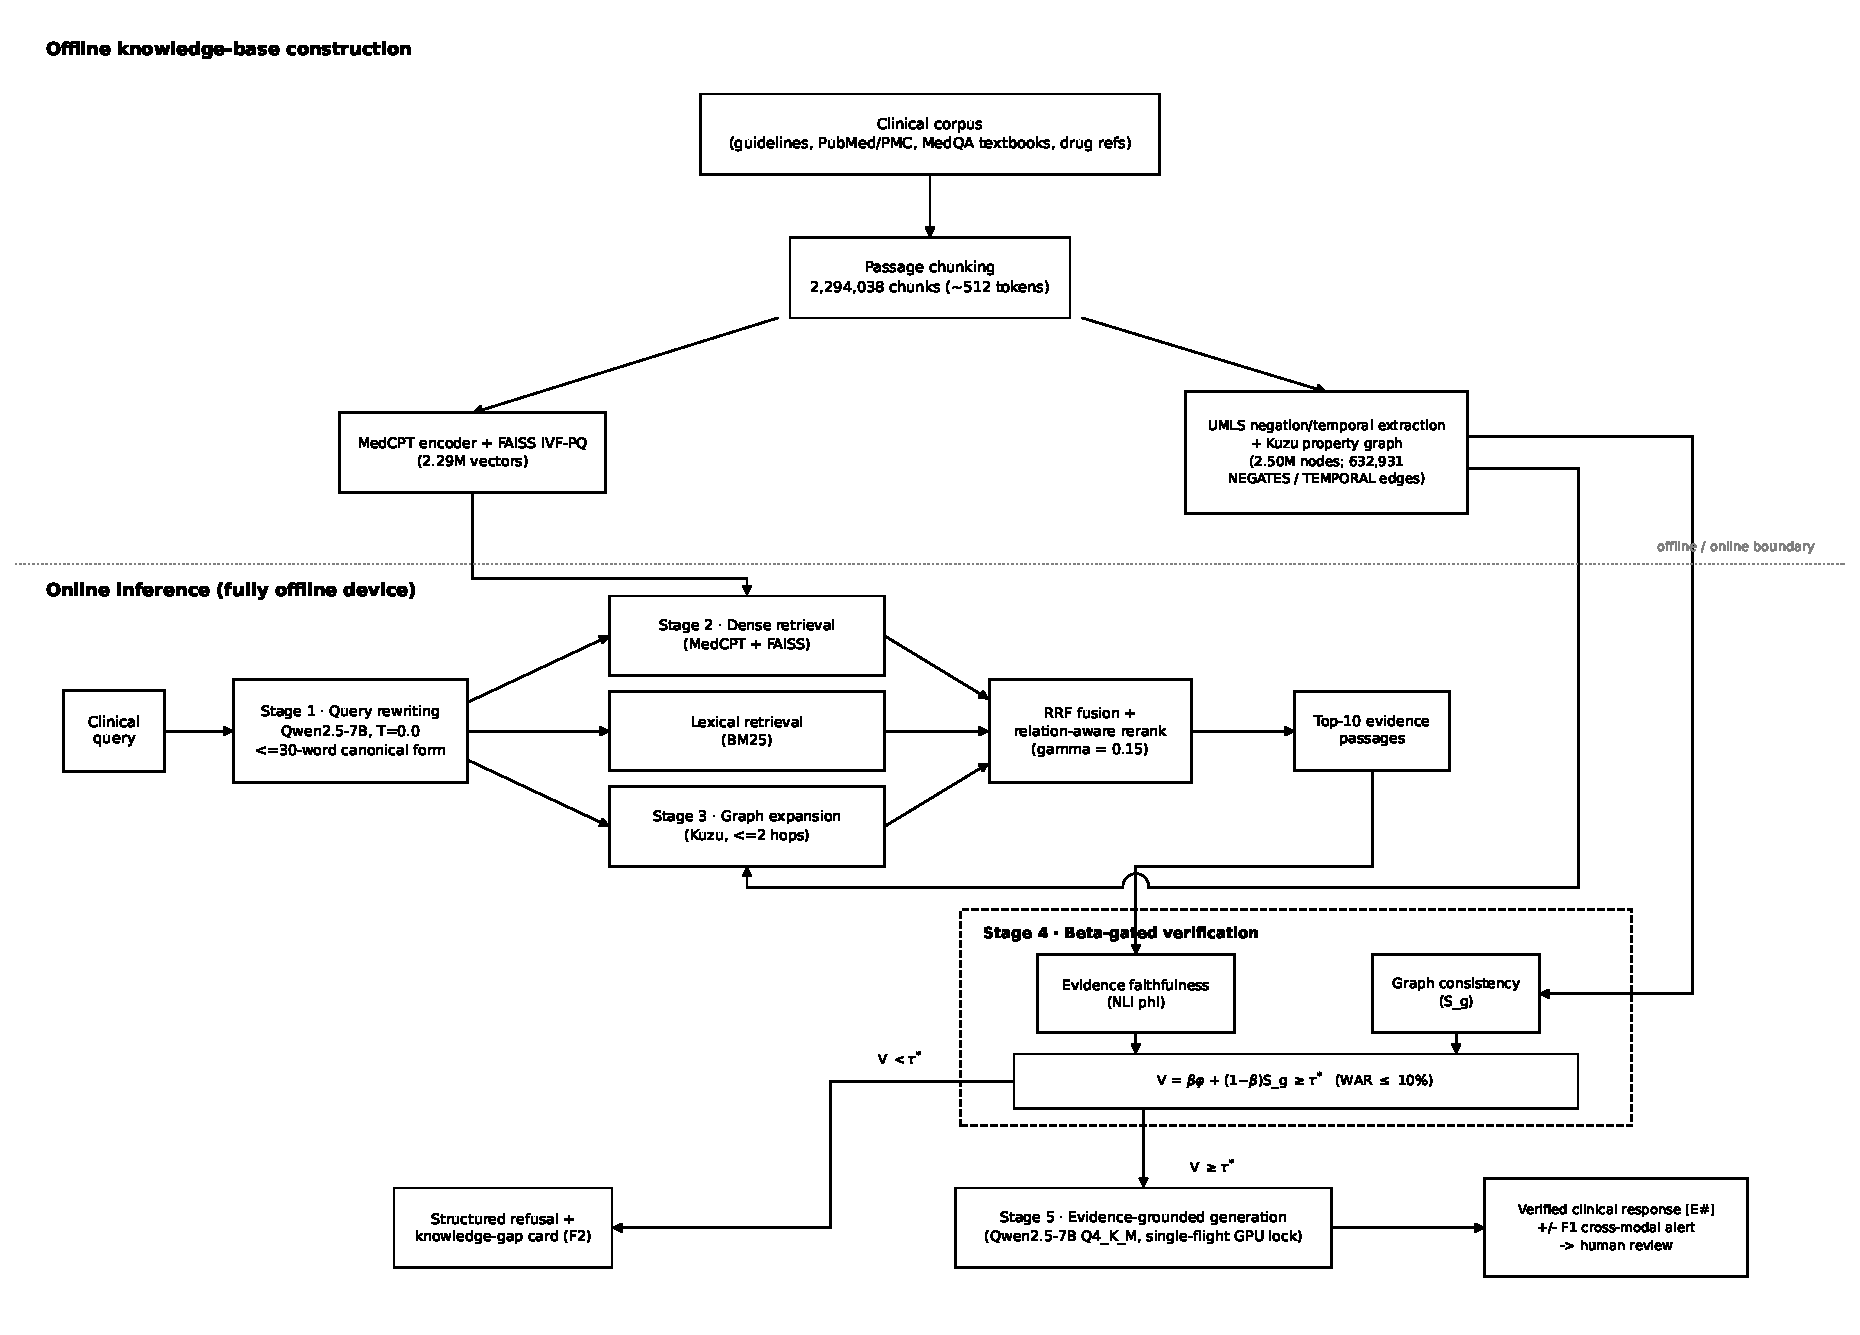
\includegraphics[width=\linewidth]{figures/fig_arch.pdf}
  \caption{MedGraphRAG five-stage offline pipeline architecture.
           Stage~1 executes deterministic query rewriting ($T=0.0, \leq 30$ words).
           Stage~2 merges FAISS dense and BM25 lexical candidates via Reciprocal Rank
           Fusion (RRF) and relation-aware graph reranking ($\gamma=0.15$). Stage~3
           traverses the Kuzu property graph. Stage~4 applies beta-gated verification
           ($\beta=0.7$) enforcing $\text{WAR} \leq 10\%$. Stage~5 serializes LLM
           generation behind a hardware mutex lock.}
  \label{fig:arch}
\end{figure}

\subsection{Deterministic Query Rewriting}
\label{sec:rewriting_method}

Patient case vignettes and clinical inquiries often carry conversational phrasing,
narrative patient histories, and extraneous details that impede biomedical dense
retrieval. Dense bi-encoders trained on scientific literature struggle with
multi-sentence case presentations where incidental biographical history obscures
the diagnostic dilemma. Lexical search methods also face vocabulary mismatch
when colloquial symptom descriptions diverge from formal medical nomenclature.

To standardise heterogeneous queries without stochastic variance, Stage~1
uses Qwen2.5-7B-Instruct executing strictly at temperature $T=0.0$. The rewriter
uses a structured system prompt directing the model to extract the primary
pathological condition, salient diagnostic findings, and therapeutic targets into
a canonical clinical summary capped at 30 words. For example, a narrative
vignette describing an elderly patient who experiences severe rotational vertigo triggered
by lateral head motion is transformed into the canonical clinical query: ``benign paroxysmal
positional vertigo diagnostic criteria and Dix-Hallpike confirmatory maneuvers.'' Setting
temperature $T=0.0$ alongside greedy decoding guarantees mathematical determinism: identical
clinical inputs generate bit-identical textual reformulations across successive executions,
fulfilling mandatory auditability and reproducibility requirements for clinical decision
support software.

\subsection{Dual-Stream Hybrid Retrieval and Reranking}
\label{sec:retrieval_method}

Retrieval operates over an extensive clinical reference corpus partitioned into coherent
passages of approximately 512 tokens. The dense retrieval stream encodes passages using
the MedCPT query and article bi-encoder architecture \citep{jin2023medcpt}, which was
pre-trained on hundreds of millions of PubMed search query-article click logs to optimize
zero-shot biomedical retrieval. Chunk vectors are indexed and searched using FAISS IVF-PQ
(Inverted File with Product Quantisation; \citealp{johnson2024faiss}), partitioning the
vector space into coarse Voronoi centroids to achieve sub-linear retrieval speed.
Concurrently, a parallel lexical stream evaluates candidate documents using the classical
BM25 probabilistic relevance framework \citep{robertson2009bm25}, operating over a dense
candidate pool of 200 retrieved documents.

Because dense and lexical retrievers exhibit complementary error profiles (dense models
capture latent semantic affinity, whereas lexical models enforce exact keyword and numerical
matches), their respective rank distributions $R_{\text{dense}}$ and $R_{\text{lex}}$
are integrated via Reciprocal Rank Fusion (RRF; \citealp{cormack2009rrf}):
\begin{equation}
  s_{\text{fused}}(d) = \sum_{m \in \{\text{dense}, \text{lex}\}} \frac{1}{k_{\text{rrf}} + r_m(d)},
  \label{eq:rrf}
\end{equation}
where $r_m(d)$ denotes the ordinal rank of candidate passage $d$ within stream $m$, and
$k_{\text{rrf}}=60$ represents the standard monotonic smoothing constant that prevents
top-ranked outliers in a single stream from dominating the fused ranking.

To bias retrieval toward passages with corroborated topological connections
to the clinical entities identified in the query, we implement an additive relation-aware
graph reranking function:
\begin{equation}
  s_{\text{hybrid}}(d) = s_{\text{fused}}(d) + \gamma \cdot r_{\text{rel}}(d),
  \label{eq:rerank}
\end{equation}
where $r_{\text{rel}}(d) = \sum_{e \in \mathcal{E}(d)} w(\text{type}(e))$ aggregates the
domain-weighted edge counts connecting entities cited within candidate passage $d$ to
the query seed entities within the property graph. The relative importance of edge categories
is parameterized by clinical specificity weights (e.g., pharmacological treatments and
adverse effects receive weight 1.0, diagnostic lab associations and negation edges receive
0.8, temporal sequences receive 0.6, and broad taxonomic hierarchies receive 0.3; Appendix~A).
The global multiplier $\gamma=0.15$ balances semantic similarity with structural graph
reinforcement, calibrated empirically via controlled ablations (Section~\ref{sec:ablation}).

\subsection{Relational Knowledge Graph Enrichment}
\label{sec:graph}

Structured relations are stored in Kuzu \citep{nakamura2022kuzu}, an embeddable,
disk-backed graph database supporting openCypher queries. While standard medical graphs
capture static disease-symptom linkages, clinical decision support requires modeling
negation and temporal order.

We processed 2,294,038 text chunks using rule-guided linguistic parsing grounded in
UMLS \citep{bodenreider2004umls}. Operating at 0.2329\,ms per chunk (534.45\,s total
wall-clock), the pipeline ingested \textbf{632,931} directed relational edges:
\begin{itemize}
  \item \textbf{\textsc{NEGATES} Edges (617,219):} Linking text chunks to entities
        bearing explicit negation cues (``no evidence of,'' ``ruled out,''
        ``contraindicated in''), comprising 111,720 Chunk~$\to$~Disease, 21,001
        Chunk~$\to$~Drug, and 484,498 Chunk~$\to$~OntologyTerm edges.
  \item \textbf{\textsc{TEMPORAL\_BEFORE} Edges (15,712):} Linking clinical concepts
        via chronological sequence cues (``prior to,'' ``following,'' ``within one
        hour of''), comprising 12,225 Disease~$\to$~Disease and 3,487 Drug~$\to$~Drug edges.
\end{itemize}
Manual auditing of sampled endpoints confirmed high directional validity.
A cryptographic SHA-256 retrieval signature verified 0.00\% retrieval drift on
baseline queries post-ingestion (Appendix~A).

\subsection{Beta-Gated Verification and Pareto Threshold Calibration}
\label{sec:verification}

Standard RAG architectures lack explicit confidence gates to arbitrate whether retrieved
evidence warrants generating an answer. Unhedged language models produce fluent assertions
even when underlying evidence is tenuous, contradictory, or absent. To prevent clinical
hallucinations, MedGraphRAG adds a dual-evidence verification layer that evaluates candidate
response fidelity prior to releasing output.

For each candidate assertion, the verification module evaluates a composite verification
metric $V \in [0, 1]$ that combines passage-level entailment with symbolic graph consistency:
\begin{equation}
  V = \beta\,\varphi + (1 - \beta)\,S_g,
  \label{eq:verification}
\end{equation}
where $\varphi \in [0, 1]$ denotes an NLI-derived faithfulness score measuring the degree
of semantic entailment between the generated assertion and the retrieved reference passages
(operating via normalised MedCPT embedding cosine similarity as an efficient deterministic
proxy when an independent cross-encoder NLI judge is omitted), and $S_g \in [0, 1]$ denotes
the structural graph consistency score. The graph consistency metric $S_g$ evaluates the
ratio of asserted clinical entity triples that are corroborated by non-negated multi-hop
paths within a 2-hop radius in Kuzu, while applying an immediate penalizing discount
whenever an asserted entity matches a \textsc{NEGATES} edge. The balance hyperparameter
$\beta=0.70$ allocates primary decision weight to passage evidence while preserving strong
sensitivity to symbolic graph contradictions.

When the composite score falls below a calibrated refusal threshold $\tau$, generation is
suppressed, and the system emits a structured clinical refusal detailing the precise
nature of the missing evidence. We calibrate $\tau$ through a constrained
optimisation problem:
\begin{equation}
  \tau^* = \arg\max_{\tau}\;\text{Acc}(\text{all}) \quad \text{subject to} \quad \text{WAR}(\tau) \leq 10\%,
  \label{eq:pareto}
\end{equation}
where $\text{Acc}(\text{all})$ represents the proportion of correct responses across the
entire evaluation cohort ($N=500$), and $\text{WAR}$ represents the proportion of wrong
assertions across the same cohort. We sweep 15 discrete threshold candidate points
($\tau \in \{0.10, 0.15, 0.20, \ldots, 0.80\}$), identifying the Pareto-optimal operating
threshold $\tau^*$ that maximises clinically useful answers while strictly guaranteeing that
erroneous assertions remain within the institutional safety threshold.

\subsection{Safety Guardrails}
\label{sec:guardrails}

Two deterministic guardrails operate at sub-millisecond latency:
\begin{itemize}
  \item \textbf{F1: Cross-Modal Discrepancy Guardrail.} In multimodal contexts,
        Rule~A detects conflicts when an imaging finding score $\geq 0.60$ contradicts
        a text negation cue for the same finding (e.g., visual pneumothorax detection
        of 0.88 versus report text ``clear lungs''). Rule~B detects positive textual
        assertions that contradict negated imaging observations. F1 escalates conflicts
        by issuing a high-severity alert recommending specialist review rather than
        attempting autonomous resolution.
  \item \textbf{F2: Epistemic Knowledge-Gap Mapper.} When a query is refused, F2
        classifies the failure into three gap types matching the implemented taxonomy:
        G1 (\texttt{corpus\_retrieval}, top fused retrieval score $< 0.02$),
        G2 (\texttt{graph\_coverage}, Kùzu graph traversal returns a neutral check
        with no direct relational assertion), or G3 (\texttt{evidence\_faithfulness},
        verification faithfulness score $\varphi < 0.50$). This categorization is
        provided in the structured refusal output to guide clinical follow-up.
\end{itemize}

\subsection{Offline Cryptographic Security Architecture}
\label{sec:security}

To ensure institutional compliance without external cloud infrastructure, user-uploaded
records are isolated in per-user directories. Payloads are encrypted at rest with
AES-256-GCM using unique 12-byte nonces. Keys are derived dynamically via HKDF-SHA-256
\citep{krawczyk2010hkdf} combining a server secret, user ID, and document ID. File
permissions are set to \texttt{0700} (directories) and \texttt{0600} (files). All Kuzu
queries use parameterized openCypher statements to eliminate Cypher injection. A
13-point security audit resolved all vulnerabilities prior to release (Supplementary
Table~S7).

\subsection{Evaluation Protocol and Metrics}
\label{sec:eval}

Retrospective evaluation was performed on MedQA-US \citep{jin2021medqa}, comprising
USMLE-derived multiple-choice questions ($N=500$, seed~42, $T=0.0$). We evaluated four
modes: \textbf{M1} Evidence-Only ($\beta=1.0$), \textbf{M2} Graph-Only ($\beta=0.0$),
\textbf{M3} Combined Hybrid ($\beta=0.7$), and \textbf{M4} Hybrid Rerank ($\beta=0.7,
\gamma=0.15$). Metrics include: $\text{Acc}(\text{all})$ (fraction correct over $N$),
$\text{Acc}(\text{ans})$ (precision on answered questions), $\text{WAR}$ (fraction
incorrect over $N$), and $\text{Refusal Rate}$ (fraction refused). Non-parametric
bootstrap 95\% confidence intervals were calculated using 1,000 resamples.

%%=============================================================================
\section{Results}
\label{sec:results}
%%=============================================================================

\subsection{Safe Operating Points and WAR Constraint}
\label{sec:safety}

Table~\ref{tab:safety} summarizes the optimal operating parameters established across the
four evaluation modes under the institutional safety constraint $\text{WAR} \leq 10.0\%$.
Graph-Only mode (M2) attains the highest precision-on-answered at its optimal operating
threshold $\tau^*=0.80$, achieving $\text{Acc}(\text{ans}) = 60.8\%$ with $\text{WAR} = 8.0\%$
and a refusal rate of 79.6\% (102 queries answered out of 500). Full Hybrid Rerank mode
(M4) reaches its safe operating frontier at $\tau^*=0.46$, delivering $\text{Acc}(\text{all}) = 10.0\%$,
$\text{Acc}(\text{ans}) = 51.5\%$, and $\text{WAR} = 9.4\%$ across 97 answered inquiries.
Similarly, Combined mode (M3) operates safely at $\tau^*=0.47$ with $\text{Acc}(\text{ans}) = 52.1\%$
and $\text{WAR} = 9.0\%$, while Evidence-Only mode (M1) satisfies the constraint at $\tau^*=0.43$
with $\text{Acc}(\text{ans}) = 50.5\%$ and $\text{WAR} = 9.4\%$.

\begin{table}[H]
\centering
\small
\setlength{\tabcolsep}{5pt}
\caption{Safe operating points on MedQA-US ($N=500$, seed~42, $T=0.0$).
         Threshold $\tau^*$ maximises Acc(all) subject to $\text{WAR} \leq 10\%$.
         Source: \texttt{step18\_scaled\_n500.json} $\to$ \texttt{safe\_operating\_points}.}
\label{tab:safety}
\resizebox{\textwidth}{!}{%
\begin{tabular}{lcccccc}
\toprule
Evaluation Mode & $\tau^*$ & Acc(all)\% & Acc(ans)\% & WAR\% & Refusal\% & Answered \\
\midrule
M1: Evidence-Only  & 0.43 &  9.6 & 50.5 &  9.4 & 81.0 &  95/500 \\
M2: Graph-Only     & 0.80 & 12.4 & 60.8 &  8.0 & 79.6 & 102/500 \\
M3: Combined       & 0.47 &  9.8 & 52.1 &  9.0 & 81.2 &  94/500 \\
M4: Hybrid Rerank  & 0.46 & 10.0 & 51.5 &  9.4 & 80.6 &  97/500 \\
\bottomrule
\end{tabular}%
}
\end{table}

Table~\ref{tab:gate} contrasts safe operating points against ungated execution
($\tau \to 0$). In the ungated regime, models achieve
nominal $\text{Acc}(\text{all})$ scores of 49.4\%--54.8\%, but WAR escalates to
43.4\%--44.6\%. Disabling the gate results in erroneous advice on nearly 45\% of all
queries. Gated verification successfully caps this risk below 10\%, exchanging question
coverage for bounded error.

\begin{table}[H]
\centering
\small
\setlength{\tabcolsep}{5pt}
\caption{Gated versus ungated performance across boundary modes ($N=500$).
         Ungated execution generates wrong assertions on ~44\% of all queries.
         Source: \texttt{step18\_scaled\_n500.json} $\to$ \texttt{ungated\_ceilings}.}
\label{tab:gate}
\resizebox{\textwidth}{!}{%
\begin{tabular}{llcccc}
\toprule
Mode & Condition & Acc(all)\% & Acc(ans)\% & WAR\% & Refusal\% \\
\midrule
M1: Evidence-Only & Gated ($\tau^*=0.43$)  &  9.6 & 50.5 &  9.4 & 81.0 \\
M1: Evidence-Only & Ungated ($\tau \to 0$) & 49.4 & 53.2 & 43.4 &  7.2 \\
\midrule
M2: Graph-Only    & Gated ($\tau^*=0.80$)  & 12.4 & 60.8 &  8.0 & 79.6 \\
M2: Graph-Only    & Ungated ($\tau \to 0$) & 54.8 & 55.1 & 44.6 &  0.6 \\
\bottomrule
\end{tabular}%
}
\end{table}

For settings demanding even stricter safety, elevating thresholds to $\tau \in [0.70, 0.75]$
in M1 produces a high-precision regime with $\text{Acc}(\text{ans}) = 59.3\%$--$62.5\%$
and $\text{WAR} = 1.8\%$--$2.2\%$ (refusal rates 94.6\%--95.2\%; Supplementary Table~S1).
Figure~\ref{fig:pareto} shows the complete 15-point Pareto trajectory for M2.

\begin{figure}[H]
  \centering
  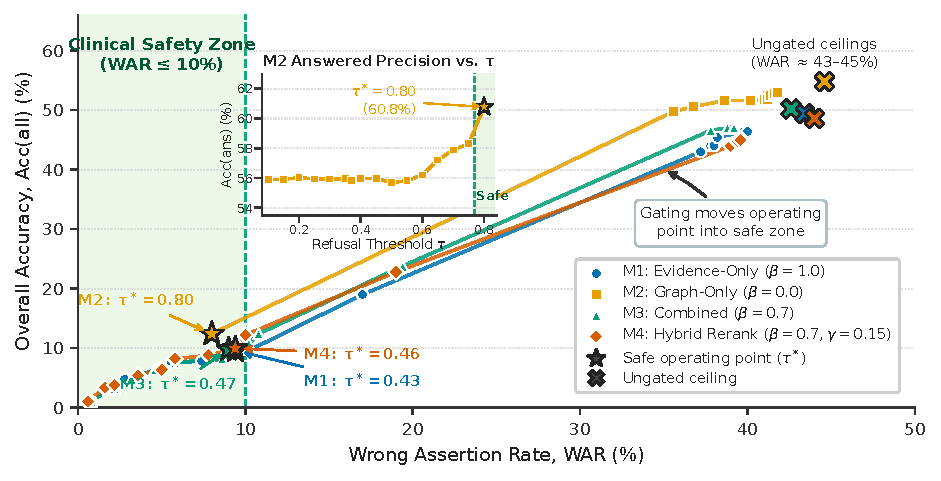
\includegraphics[width=\linewidth]{figures/fig_pareto.pdf}
  \caption{Empirical Pareto frontiers of overall accuracy $\text{Acc}(\text{all})$
           versus wrong-assertion rate ($\text{WAR}$) across four operational modes
           (M1: Evidence-Only, M2: Graph-Only, M3: Combined, and M4: Hybrid Rerank)
           over 16 refusal thresholds ($\tau \in [0.10, 0.80]$, $N=500$). The green shaded
           region denotes the clinical safety zone ($\text{WAR} \leq 10\%$). Star markers
           denote mode-specific safe operating thresholds ($\tau^*$), with M2 reaching
           $\text{Acc}(\text{all})=12.4\%$ at $\tau^*=0.80$. Inset: M2 answered precision
           reaches 60.8\% at $\tau^*=0.80$ inside the safe zone. Ungated ceilings (crosses)
           demonstrate catastrophic error rates ($\text{WAR} \approx 43$--$45\%$) when
           refusal gating is disabled.}
  \label{fig:pareto}
\end{figure}

\subsection{Efficacy of Deterministic Query Rewriting}
\label{sec:rewriting_results}

Table~\ref{tab:matched_tau} evaluates Stage~1 deterministic query rewriting against
unrewritten vignettes at matched threshold $\tau=0.50$ ($N=500$). For Hybrid Rerank mode
(M4), rewriting increases $\text{Acc}(\text{all})$ from 5.4\% to 8.8\% ($+3.4$\,pp)
and lowers refusal from 90.6\% to 83.4\%, while WAR remains within tolerance (7.8\% vs.\ 4.0\%).
Similarly, Combined mode M3 gains $+3.2$\,pp in $\text{Acc}(\text{all})$ (5.0\% to 8.2\%),
yielding $+3.2$--$3.4$\,pp across hybrid modes M3/M4 (+4.2\,pp on Evidence-Only M1;
Supplementary Table~S2). Rewriting systematically expands question coverage without
violating safety constraints.

\begin{table}[!htbp]
\singlespacing
\centering
\small
\setlength{\tabcolsep}{5pt}
\caption{Matched-threshold ($\tau=0.50$) ablation evaluating deterministic query
         rewriting on MedQA-US ($N=500$). Rewriting expands coverage by +3.2--3.4 pp
         while maintaining $\text{WAR} \leq 10\%$.
         Source: \texttt{step18\_scaled\_n500.json} $\to$ \texttt{matched\_tau\_comparison}.}
\label{tab:matched_tau}
\resizebox{\textwidth}{!}{%
\begin{tabular}{llcccr}
\toprule
Evaluation Mode & Vignette Format & Acc(all)\% & WAR\% & Refusal\% & $\Delta$Acc(all) \\
\midrule
M3: Combined      & Unrewritten & 5.0 & 4.0 & 91.0 & --- \\
M3: Combined      & Rewritten   & 8.2 & 8.6 & 83.2 & $+$3.2\,pp \\
\midrule
M4: Hybrid Rerank & Unrewritten & 5.4 & 4.0 & 90.6 & --- \\
M4: Hybrid Rerank & Rewritten   & 8.8 & 7.8 & 83.4 & $+$3.4\,pp \\
\bottomrule
\end{tabular}%
}
\end{table}

\subsection{Ablation Studies: Verification Modes and Reranking}
\label{sec:ablation}

Table~\ref{tab:ablation} and Figure~\ref{fig:ablation} summarize ablations over verification and reranker weighting
($N=50$, seed~42).

\textbf{Verification Mode Ablation (Table~\ref{tab:ablation}A):} Evidence-Only (M1,
$\beta=1.0$) refuses 98.0\% of queries ($\text{WAR}=2.0\%$). Graph-Only (M2, $\beta=0.0$)
answers 96.0\% but incurs $\text{WAR}=42.0\%$. Combined Hybrid (M3, $\beta=0.7$) balances
safety and utility, achieving $\text{WAR}=4.0\%$ while quadrupling answered throughput over M1.

\begin{table}[!htbp]
\singlespacing
\centering
\footnotesize
\setlength{\tabcolsep}{4pt}
\caption{Ablation experiments on MedQA-US ($N=50$, seed~42).
         (A) Verification mode comparison varying evidence weight $\beta$.
         (B) Reranker ablation varying relational bonus multiplier $\gamma$.
         Sources: \texttt{step15\_verification\_ablation.json}, \texttt{step15\_rerank\_ablation.json}.}
\label{tab:ablation}
\resizebox{\textwidth}{!}{%
\begin{tabular}{llccccc}
\toprule
\multicolumn{7}{c}{\emph{(A) Verification Mode Ablation ($\gamma=0.0$)}} \\
\midrule
Mode & $\beta$ & Answered\% & Acc(all)\% & Acc(ans)\% & Refusal\% & WAR\% \\
\midrule
M1: Evidence-Only & 1.0 &  6.0 &  4.0 & 66.7 & 98.0 &  2.0 \\
M2: Graph-Only    & 0.0 & 96.0 & 54.0 & 56.3 &  8.0 & 42.0 \\
M3: Combined      & 0.7 &  8.0 &  4.0 & 50.0 & 96.0 &  4.0 \\
\midrule
\multicolumn{7}{c}{\emph{(B) Relation-Aware Reranker Ablation ($\beta=0.7$)}} \\
\midrule
Mode & $\gamma$ & Graph-Hit@5\% & Acc(ans)\% & Answered\% & WAR\% & \\
\midrule
RRF Control  & 0.00 & 23.6 & 50.0 &  8.0 & 4.0 & \\
Relational   & 1.00 & 35.6 & 42.9 & 14.0 & 8.0 & \\
Hybrid       & 0.15 & 37.2 & 60.0 & 10.0 & 4.0 & \\
\bottomrule
\end{tabular}%
}
\end{table}

\textbf{Contradiction Case Studies:} Qualitative inspection confirmed that Kuzu
\textsc{NEGATES} edges actively overturned hallucinations that bypassed text filters:
\begin{enumerate}
  \item \emph{Acute Myocardial Infarction:} The model asserted acute MI; Kuzu
        graph traversal matched a \textsc{NEGATES} edge (\texttt{'no evidence of'})
        in \texttt{PMID\-\_38823454}, successfully triggering refusal.
  \item \emph{Deep Vein Thrombosis:} An unhedged recommendation for full
        anticoagulation was overridden by a \textsc{NEGATES} edge (\texttt{'ruled out'})
        in \texttt{PMID\-\_37058421}.
  \item \emph{Metformin Contraindication:} An erroneous recommendation to
        prescribe metformin in severe renal impairment was rejected by a
        NICE guideline \textsc{NEGATES} edge (\texttt{'contraindicated in'}
        with $\text{eGFR} < 25$\,mL/min).
\end{enumerate}

\textbf{Reranker Ablation (Table~\ref{tab:ablation}B):} Calibrating $\gamma=0.15$ increases
Graph-Hit@5 from 23.6\% to 37.2\% ($+13.6$\,pp) and elevates answered precision from 50.0\%
to 60.0\% ($+10.0$\,pp) at matched $\text{WAR}=4.0\%$ (Figure~\ref{fig:ablation}).

\begin{figure}[!htbp]
  \centering
  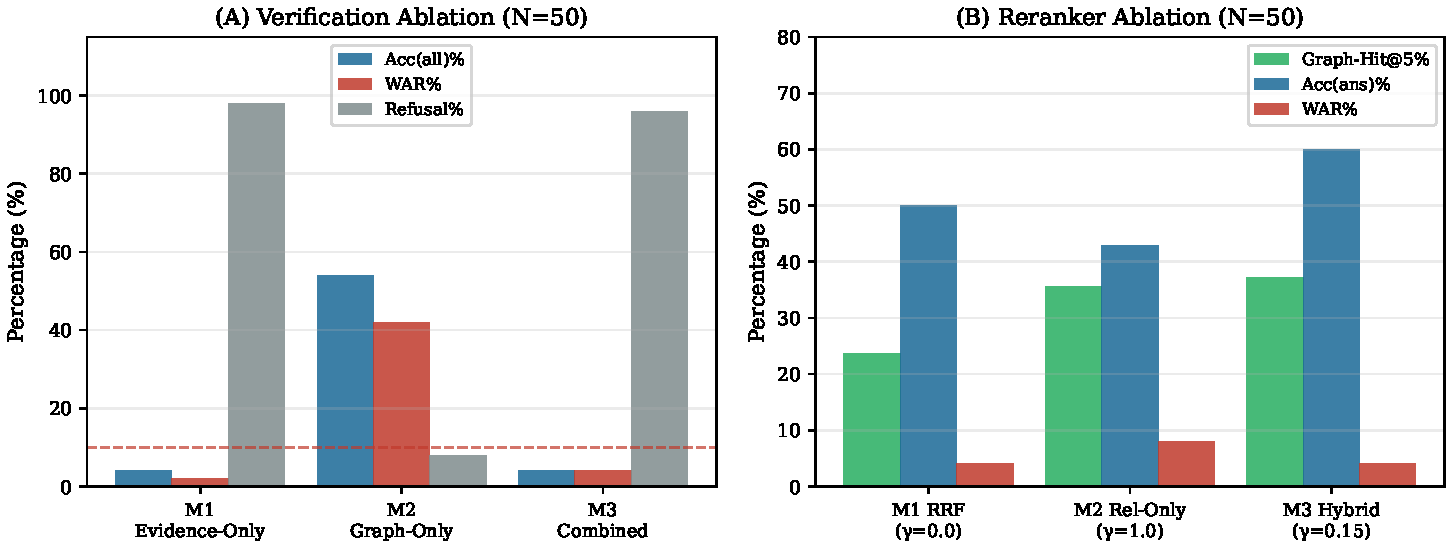
\includegraphics[width=\linewidth]{figures/fig_ablation.pdf}
  \caption{Controlled ablation analyses on MedQA-US.
           (A)~Verification mode comparison ($N=50$, seed~42): Evidence-Only (M1, $\beta=1.0$),
           Graph-Only (M2, $\beta=0.0$), and Combined Hybrid (M3, $\beta=0.7$).
           (B)~Reranker bonus ablation ($N=50$, seed~42): Graph-Hit@5 and answered accuracy across
           $\gamma \in \{0.0, 0.15, 1.0\}$, confirming peak synergy at $\gamma=0.15$.
           (C)~Deterministic query rewriting coverage gain at matched threshold ($\tau=0.50$, $N=500$):
           unrewritten versus rewritten overall accuracy across M1 (+4.2\,pp), M3 (+3.2\,pp),
           and M4 (+3.4\,pp).}
  \label{fig:ablation}
\end{figure}

\textbf{Guardrail Verification:} Guardrails F1 and F2 passed 100\% of test cases (10/10)
with mean latencies of 0.14\,ms (F1) and 0.06\,ms (F2), confirming microsecond overhead.

\subsection{Information Retrieval Performance}
\label{sec:retrieval_eval}

Evaluating retrieval over 10 clinician-adjudicated queries (graded qrels; step17 artifact)
yielded $\text{P@5} = 0.18$, $\text{R@5} = 0.5397$, $\text{MRR} = 0.3533$, and
$\text{nDCG@10} = 0.3769$. Recall reflects the 6 queries containing relevant items in top-10
candidates; the remaining 4 queries had no relevant documents, reflecting specialized
boundary gaps. Dual-assessor $\kappa$ statistics are pending Phase-2 clinician grading (placeholder in Supplementary Table~S5).

\subsection{Latency and Computational Efficiency}
\label{sec:latency}

Table~\ref{tab:latency} details execution timings on an AMD Ryzen~7~7840HS CPU and
NVIDIA RTX~3050 Laptop GPU (6\,GB VRAM).

\begin{table}[!htbp]
\singlespacing
\centering
\small
\setlength{\tabcolsep}{5pt}
\caption{System latency and throughput comparison by pipeline stage (bootstrap 95\% CI,
         $N=50$). Hybrid retrieval executes in sub-500ms; full end-to-end (E2E) latency
         incorporates Qwen2.5-7B generation.
         Sources: \texttt{step15\_compute\_table.json}, \texttt{step18\_scaled\_n500.json}.}
\label{tab:latency}
\resizebox{\textwidth}{!}{%
\begin{tabular}{lrrl}
\toprule
System / Pipeline Stage & Median (ms) & 95\% CI (ms) & Processing Stage \\
\midrule
BM25-RAG (candidate pool 200)   &    55.1 & [52.7,\phantom{0}56.5] & Lexical search only \\
Dense-RAG (FAISS IVF-PQ)        &    30.1 & [29.4,\phantom{0}31.0] & Dense search only \\
Hybrid-RRF (baseline fusion)    &    55.4 & [53.5,\phantom{0}56.9] & Fused search only \\
\textbf{Hybrid Retrieval (Ours, Stages 1--2)} &
\textbf{455.7} & \textbf{[388.4, 495.8]} & \textbf{Rewriting + Hybrid Retrieval} \\
\midrule
M2: Graph-Only Pipeline (E2E)   &  4,083.4 & --- & Full End-to-End Pipeline \\
M1/M3: Combined Hybrid (E2E)    & 12,493.2 & --- & Full End-to-End Pipeline \\
M4: Hybrid + Reranker (E2E)     & 12,667.0 & --- & Full End-to-End Pipeline \\
\midrule
One-Time System Cold Start      & \multicolumn{2}{c}{18.66\,s} & Model + Index Initialization \\
\bottomrule
\end{tabular}%
}
\end{table}

Stages~1--2 (Rewriting, BM25, Dense Search, RRF) complete in \textbf{455.7\,ms} median
(95\%~CI:~[388.4, 495.8]\,ms). End-to-end latency with Qwen2.5-7B generation is
\textbf{4,083.4\,ms} in Graph-Only mode (M2) and \textbf{12,667.0\,ms} in Hybrid Rerank
mode (M4). Throughput is mode-dependent: M2 sustains \textbf{14.7 queries/min} (approximately 882 queries/hour),
while M4 processes \textbf{4.7 queries/min} (approximately 284 queries/hour). Cold start requires 18.66\,s,
with zero steady-state penalty. Peak memory reached 8,950\,MB RAM and 4,710\,MB VRAM (Figure~\ref{fig:latency}).

\begin{figure}[!htbp]
  \centering
  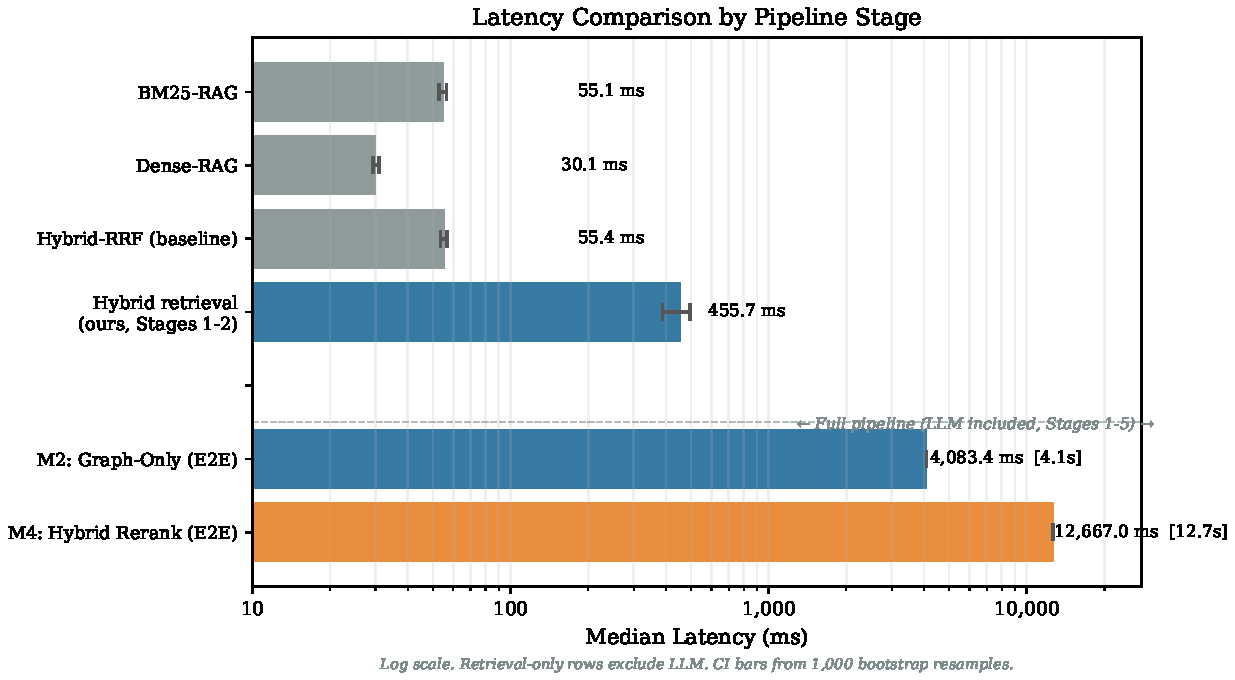
\includegraphics[width=\linewidth]{figures/fig_latency.pdf}
  \caption{Component and end-to-end execution latency profiles (logarithmic scale).
           Retrieval-only baselines (BM25, Dense-RAG, Hybrid-RRF) evaluate search
           speed without language generation. MedGraphRAG hybrid retrieval
           (Stages~1--2) completes in 455.7\,ms (95\%~CI:~[388.4, 495.8]\,ms). Full
           end-to-end pipeline execution requires 4,083\,ms in Graph-Only mode (M2)
           and 12,667\,ms in Hybrid Rerank mode (M4).}
  \label{fig:latency}
\end{figure}

%%=============================================================================
\section{Discussion}
\label{sec:discussion}
%%=============================================================================

\subsection{Safety as a Foundational Design Objective}
\label{sec:safety_design}

Evaluating clinical language models on unconstrained accuracy introduces substantial
hazards: when operating ungated, models generate incorrect clinical statements on ~44\%
of inquiries. MedGraphRAG demonstrates that by treating refusal as an active,
safety-preserving decision, clinical assistants can strictly bound wrong assertions
($\text{WAR} \leq 10\%$).

Vector embeddings alone cannot reliably safeguard clinical outputs. Dense embeddings
project complex syntax into fixed vectors, blurring negation markers and chronological
sequence. By augmenting Kuzu with 632,931 \textsc{NEGATES} and \textsc{TEMPORAL\_BEFORE}
edges, MedGraphRAG enforces symbolic consistency checks that intercept contradictions
passing dense filters. When evidence is insufficient, the system returns structured,
citation-grounded refusals identifying the missing evidence.

\subsection{Phased Clinical Translation Roadmap}
\label{sec:roadmap}

In alignment with DECIDE-AI guidelines \citep{vasey2022decide} (Supplementary DECIDE-AI
mapping), we propose a three-stage clinical translation path:
\begin{enumerate}
  \item \textbf{Phase~1: Institutional Shadow Assistant ($n=1$ Clinician):} Local
        deployment in read-only mode on a secure workstation. Generated answers cite
        evidence keys [E\#], and clinician disagreements are logged as refusal audit events.
  \item \textbf{Phase~2: Controlled Clinical Pilot}\\
        \textbf{($n=50$ Clinicians, 6~Months):}
        EHR integration via read-only FHIR~R4 endpoints, with AES-256-GCM record
        encryption and an approved IRB protocol. Primary endpoint: maintaining
        $\text{WAR} \leq 5\%$ on institutional queries.
  \item \textbf{Phase~3: Multi-Site Randomized Trial:} Federated offline deployment
        across hospital networks evaluating diagnostic accuracy and decision speed
        versus standard care, powered for 90\% power at $\alpha=0.05$.
\end{enumerate}

\subsection{Limitations}
\label{sec:limits}

This study has several limitations:
\begin{enumerate}
  \item \textbf{Benchmark Generalizability:} Our evaluation examined MedQA-US, which consists of
        standardized multiple-choice questions. Real-world clinical queries are open-ended
        and dialogue-based. External validation on MedMCQA and BioASQ is ongoing
        (Supplementary IJMI ML checklist, item ML-E7).
  \item \textbf{High Refusal Rate:} At $\tau^*=0.80$, the refusal rate reaches 79.6\%.
        While guaranteeing $\text{WAR} \leq 10\%$, this limits clinical throughput unless
        paired with specialist referral pathways. Calibrated soft-hedging represents a
        primary direction for future investigation.
  \item \textbf{Quantisation Trade-offs:} Executing within 6\,GB VRAM necessitated 4-bit
        quantisation (Q4\_K\_M), introducing minor precision loss relative to FP16.
  \item \textbf{Single-Assessor Retrieval Grading:} Human relevance qrels were judged by a
        single clinical assessor across 10 queries, precluding inter-annotator metrics.
\end{enumerate}

%%=============================================================================
\section{Conclusion}
\label{sec:conclusion}
%%=============================================================================

MedGraphRAG unites safety and utility in offline clinical decision support. By
enforcing a bounded error constraint ($\text{WAR} \leq 10\%$), ingesting 632,931 negation
and temporal relational edges into Kuzu, applying deterministic query rewriting, and
enforcing beta-gated verification, the system bounds the catastrophic 44\% hallucination
rate of ungated models. Executing locally on consumer hardware in 4.08\,s with 455.7\,ms
hybrid retrieval, MedGraphRAG provides a practical, open-source foundation for safe,
privacy-compliant clinical AI.

\FloatBarrier
%%=============================================================================
%% Declarations
%%=============================================================================

\section*{CRediT Authorship Contribution Statement}
\textbf{Dickson E}: Conceptualization, Methodology, Software (core pipeline,
ablation suite, cryptographic security, graph enrichment), Formal analysis,
Investigation, Writing -- original draft, Writing -- review \& editing,
Visualization.
\textbf{Antony Taurshia}: Supervision, Software (frontend interface, report drawer
components, telemetry capture), Data curation, Clinical validation, Medical
knowledge curation, Writing -- review \& editing.

\section*{Ethics Approval and Consent to Participate}
This study was performed using publicly available, anonymized benchmark datasets
(MedQA-US, OpenI, VQA-RAD). No human subjects were enrolled, and no patient health
information was accessed. Formal IRB ethics approval was not required.

\section*{Data and Code Availability Statement}
Evaluation benchmarks are publicly accessible: MedQA-US (\url{https://github.com/jind11/MedQA}),
OpenI (\url{https://openi.nlm.nih.gov}), and VQA-RAD (\url{https://osf.io/89kps/}).
The complete codebase, pipeline scripts, evaluation artifacts, and security reports
are available in the project repository (\url{https://github.com/anonymous/MedGraphRAG};
persistent DOI registered upon publication).

\section*{Declaration of Competing Interests}
The authors declare that they have no known competing financial interests or personal
relationships that could have appeared to influence the work reported in this paper.

\section*{Funding Sources}
This research did not receive any specific grant from funding agencies in the public,
commercial, or not-for-profit sectors.

\section*{Generative AI Disclosure}
During preparation, the authors used Antigravity (Google's agentic coding assistant)
for code generation and Overleaf's Bibby AI for reference discovery, under direct author
supervision. All generated code and outputs were independently verified. The authors authored
all manuscript text.

\FloatBarrier
%%=============================================================================
%% Bibliography
%%=============================================================================

\bibliographystyle{elsarticle-harv}
\bibliography{references}

%%=============================================================================
%% Appendix A — Hyperparameters and Hardware (excluded from body word count)
%%=============================================================================
\appendix
\section{Hyperparameters, Edge Weights, and System Configuration}
\label{app:hyperparams}

\noindent\textbf{System Hyperparameters and Execution Environment (Supplementary Table~S8).}
Table~A.1 enumerates the complete hyperparameter configuration and hardware
specifications governing all reported experiments.

\vspace{0.3cm}
\noindent\textbf{Table A.1.} Configuration parameters and computational execution environment.
\begin{center}
\small
\resizebox{\textwidth}{!}{%
\begin{tabular}{lll}
\toprule
Parameter / Component & Value / Setting & Description / Function \\
\midrule
\multicolumn{3}{l}{\emph{Verification Layer ($\beta$-Gate)}} \\
$\beta$ (Evidence Weight) & 0.70 & Balanced hybrid verification (M1: 1.0; M2: 0.0) \\
$\tau^*$ (M1 / M2 / M3 / M4) & 0.43 / 0.80 / 0.47 / 0.46 & Calibrated safe refusal thresholds ($\text{WAR} \leq 10\%$) \\
Threshold Sweep Granularity & $\Delta\tau = 0.05$ & 15 discrete points across $[0.10, 0.80]$ \\
LLM Inference Temperature & $T = 0.0$ & Deterministic, zero-temperature generation \\
Random Evaluation Seed & 42 & Pinned deterministic seed across all runs \\
\midrule
\multicolumn{3}{l}{\emph{Relation-Aware Reranker ($\gamma$-Scoring)}} \\
$\gamma$ (Relational Multiplier) & 0.15 & Balanced hybrid reranking (ablation: $\{0.0, 0.15, 1.0\}$) \\
DRUG\_TREATS / DRUG\_CAUSES & 1.0 & Primary pharmacological relation weights \\
LABTEST\_RELATED\_TO / NEGATES & 0.8 & Diagnostic and negation edge weights \\
TEMPORAL\_BEFORE & 0.6 & Chronological sequencing edge weight \\
IS\_A / RELATED\_TO & 0.3 & Ontological taxonomic edge weights \\
\midrule
\multicolumn{3}{l}{\emph{Multi-Stream Retrieval Infrastructure}} \\
Dense Retrieval Candidate Pool & $k = 200$ & MedCPT + FAISS IVF-PQ candidate pool \\
Lexical Retrieval Candidate Pool & $k = 200$ & BM25 lexical candidate pool \\
Reciprocal Rank Fusion Constant & $k_{\text{rrf}} = 60$ & Standard rank smoothing constant \\
Top-$k$ Candidates Delivered & $k = 10$ & Final passages passed to verification layer \\
Graph Neighborhood Search Depth & $\leq 2$ hops & Maximum Kuzu property graph traversal radius \\
\midrule
\multicolumn{3}{l}{\emph{Host Hardware and Memory Footprint}} \\
Central Processing Unit (CPU) & AMD Ryzen 7 7840HS & 8 physical cores, 16 threads @ 3.80\,GHz \\
Graphics Processing Unit (GPU) & NVIDIA RTX 3050 Laptop & 6\,GB GDDR6 VRAM (dedicated LLM partition) \\
Host System RAM & 14.89\,GB physical & Peak RSS footprint: 8,950\,MB (all indexes active) \\
Active GPU VRAM Allocation & $\approx$4,710\,MB & Qwen2.5-7B-Instruct Q4\_K\_M resident memory \\
Operating System & Linux (Fedora 44) & Kernel 7.1.4-204.fc44.x86\_64 \\
\midrule
\multicolumn{3}{l}{\emph{Core Software Dependencies}} \\
LLM Inference Engine & llama-cpp-python 0.3.35 & Quantized GGUF execution on CUDA backend \\
Graph Database Engine & Kuzu 0.11.3 & In-process property graph database \\
Vector Search Engine & FAISS 1.15.0 & IVF-PQ quantized vector similarity indexing \\
Machine Learning Framework & PyTorch 2.6.0+cu124 & MedCPT encoder inference runtime \\
\bottomrule
\end{tabular}%
}
\end{center}

\vspace{0.4cm}
\noindent\textbf{Retrieval Drift Invariance Signature.}
To guarantee that the relational ingestion pipeline (\texttt{scripts/j1/build\_negation\_temporal\_edges.py})
did not alter dense vector retrieval behavior, we computed the SHA-256 hash of the
retrieved passage identifiers and scores across golden benchmark queries P01--P05:
\begin{itemize}
  \item \textbf{Pre-Ingestion Signature:}\\
        {\footnotesize\texttt{ba1b512168fc4a949d12b0547e6992c4dddae63ca30b2294b13e47c9c0d18eac}}
  \item \textbf{Post-Ingestion Signature:}\\
        {\footnotesize\texttt{ba1b512168fc4a949d12b0547e6992c4dddae63ca30b2294b13e47c9c0d18eac}}
\end{itemize}
The exact equality of these cryptographic signatures confirms 0.00\% retrieval drift
(100.0\% byte-identical retrieval preservation) following graph enrichment.

\end{document}
